\section{Figures moved from the main text}
\label{sec:supp_moved}
To keep the revised manuscript short, four figures of the submitted version were moved here. Their data are
unchanged; Fig.~S6 shows the revised delayed-feedback controller.

\begin{figure}[!t]
\centering
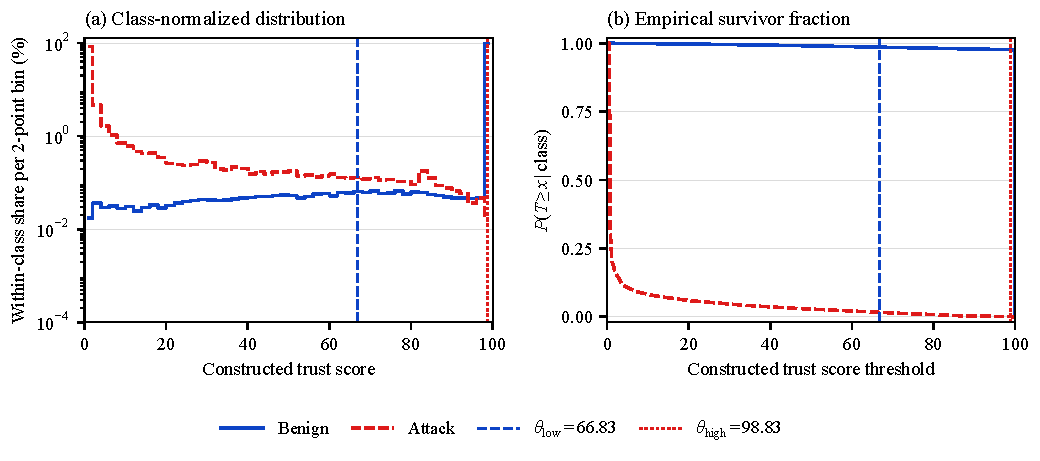
\includegraphics[width=\textwidth]{figures/main_fig_trust_scores.pdf}
\caption{Calibrated-HGB trust scores on the 762,000-flow test: (a) class-normalized 2-point-bin shares on a log scale and (b) empirical survivor fractions. The classes contain 613,448 benign and 148,552 attack-labeled records. Vertical lines mark the validation-selected hysteresis thresholds 66.83 and 98.83. Empty bins are retained as zeros in the source CSV.}
\label{fig:s8_trust_empirical}
\end{figure}

\begin{figure}[!t]
\centering
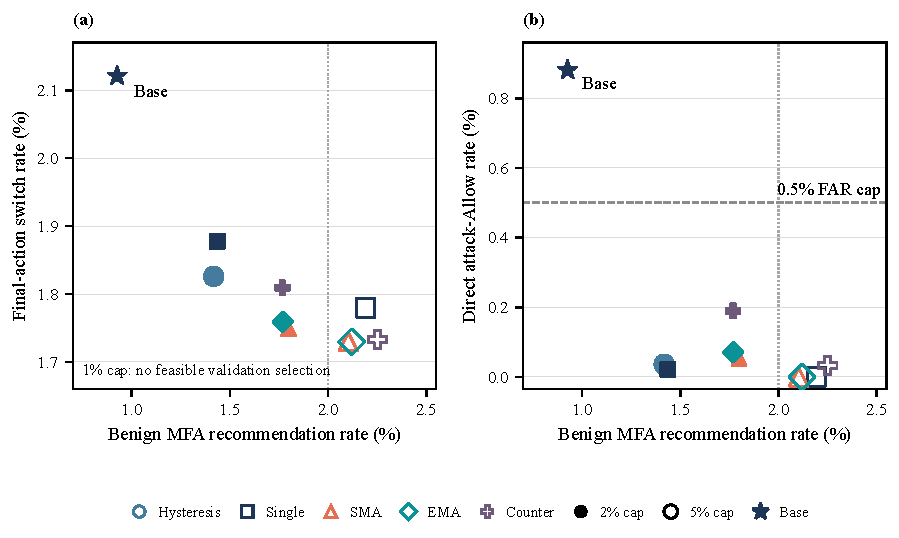
\includegraphics[width=\textwidth]{figures/main_fig_static_tradeoff.pdf}
\caption{Test rates of all policies selected on validation. Marker shapes mark the families; filled and open markers mark the 2\% and 5\% benign-MFA caps. Hysteresis selects the same pair at both caps. The dashed line is the 0.5\% direct-FAR limit. No policy is feasible on validation at the 1\% cap.}
\label{fig:s8_tradeoff_empirical}
\end{figure}

\begin{figure}[!t]
\centering
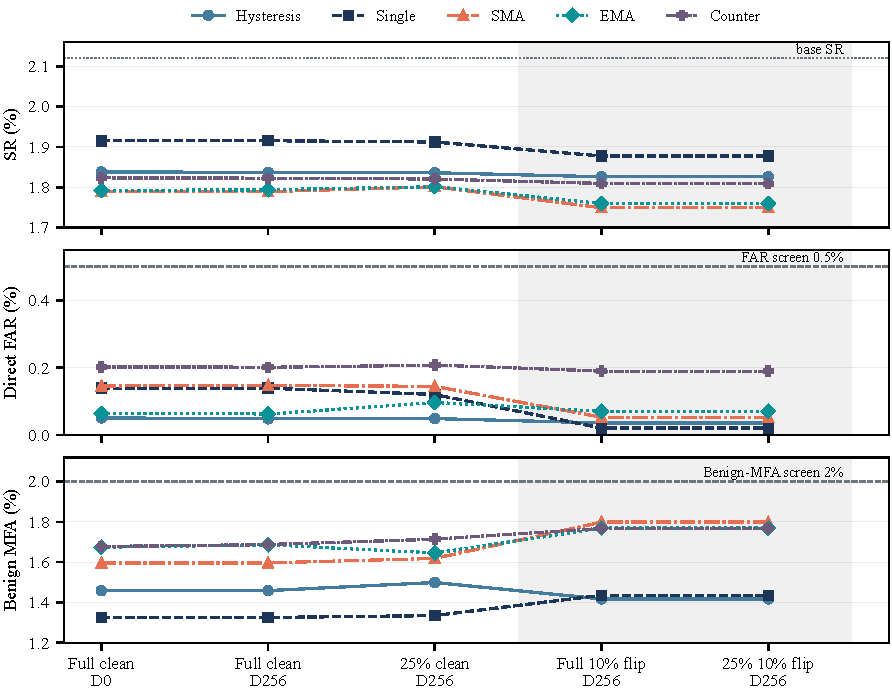
\includegraphics[width=\textwidth,height=5.8in,keepaspectratio]{figures/main_fig_feedback_conditions_R1.pdf}
\caption{All five policy families at the 2\% benign-MFA cap under the five feedback conditions, with the revised controller that starts from and returns to the validation-selected configuration. The panels show final-action SR, direct FAR and benign MFA. D0 and D256 are label delays, and 25\% clean means partial coverage. The shaded conditions add 10\% symmetric label flips. With raw window rates no update is committed in these conditions, so each family keeps its validated configuration. Dashed lines mark the limits and the base SR.}
\label{fig:s8_feedback_empirical}
\end{figure}

\begin{figure}[!t]
\centering
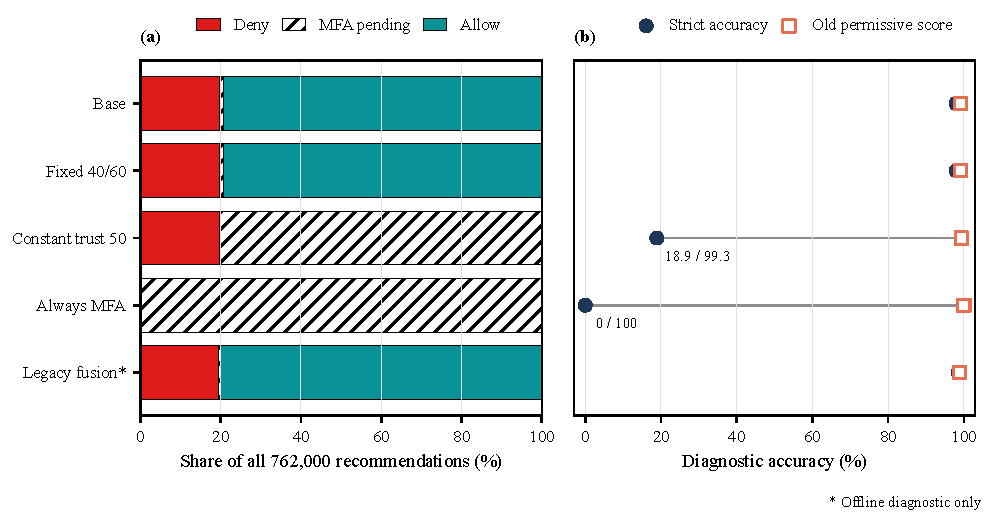
\includegraphics[width=\textwidth]{figures/main_fig_ablation.pdf}
\caption{Action mix and accuracy diagnostics on the same test. (a) Shares of Deny, pending MFA and Allow among all 762,000 recommendations. (b) Strict accuracy compared with the old permissive score that also counted MFA as correct. Always-MFA has 0\% strict and 100\% permissive accuracy, and a constant trust of 50 has 18.9\% and 99.3\%. The legacy fusion is evaluated offline only.}
\label{fig:s8_ablation_empirical}
\end{figure}

\clearpage
